\selectlanguage{english}
%%%%%%%%%%% Capitulo 2 Metodologia %%%%%%%%%%%%%%%%%%%%%%%%%%%%%%%%%%%%%%%%%%%%%%%%%%%%%%%
\setcounter{chapter}{0}
\chapter[Introduction]{Introduction}\label{c1:intro}
As you read over these lines a significant amount of the energy used by the light-bulb 
illuminating these pages is produced by the splitting of 
uranium and plutonium nuclei. 20\% if you are right now in Spain, the USA or 
the United Kingdom, 30-40\% if you are in the Czech Republic, Finland, Belgium, South Korea, 
Sweden or Switzerland and a world record of 77\% produced by state-owned company if you are 
in France.\cite{NuclearElectricEnergy} Even if you are reading this from Italy where nuclear 
energy has been forbidden, part of the energy you are consuming is nuclear since it is bought from 
the French nuclear 
industry.

Regardless of 
the reader's opinion on the nuclear power industry, it undoubtedly is an industrial leviathan 
that should be understood if only for the sake of nuclear security.  In this chapter we will 
make an effort to overview some aspects of the industry and how understanding the 
chemical nature of some of its essential substances is still relevant 70 years after the first 
nuclear reactor developed by Enrico Fermi himself. 

\section{Nuclear Power}

In 1939, Otto Hanh, Lise Meitner  and Otto Robert Frisch discovered and described the fission 
of uranium on the basis of the ``liquid drop'' model of the nucleus. Hanh
received the Nobel Prize in Chemistry for the experimental discovery. Unfortunately Meitner 
and Frisch who explained the physics behind did not. The essential idea of fission is that the 
nucleus of \ufis is metastable and the impact of a slow neutron can split it into more stable 
smaller 
nuclei. The sum of daughter nuclei masses is lower than that of \ufis \newline and 
the difference in mass is converted into tremendous amounts of energy according to Einstein's 
famous equation: $E=mc^2$. Two or three neutrons are also emitted in the process which 
depending on their speed might impact another \ufis nucleus and continue the chain reaction 
over and over.

If the concentration of \ufis is extremely high the reaction advances exponentially leading
to a sudden splitting of all the fissile nuclei and a nuclear explosion occurs. To obtain 
this critical concentration of the nuclear material generally, another conventional explosion 
must be used to compress the nuclear explosive. This is the basis of a fission nuclear bomb: 
an explosion within the bomb compresses the fissile material (uranium or plutonium) into 
critical density which releases in a split second most of its nuclear energy. This was the 
mechanism used in the bombings of Hiroshima and Nagasaki during World War II. 

The energy of fission can also be used to generate electricity by controlling the 
nuclear reaction. Uranium or plutonium act as fuel and not as explosives. The nuclear fuel is 
composed in most cases of \ce{UO2}(s) with varying ratios of \ufis/\unofis. At ordinary 
densities it generates no energy. Spontaneous fission of \ufis generates 
neutrons that are fast and inefficient in splitting other nuclei. But if we introduce a 
moderator material (typically graphite, water or heavy water) the neutrons can scatter on the 
nuclei of the moderator slowing them down and making the thermal (slow) neutrons effective in 
splitting fissile 
nuclei. This promotes fission and a chain nuclear reaction is formed generating energy. The 
growth of the energy emitted is exponential and must be reduced. For this, another material 
captures the excess neutrons and reduces the rate of fission controlling the reaction and 
avoiding a nuclear accident. These materials are substances that are effective in capturing 
neutrons, for example cadmium or boron, and are know as control materials. In this way, the fuel is 
steered 
into steady reaction. The energy liberated heats water surrounding the reactor 
vessel which in the form of steam moves turbines and a generator converts the kinetic energy 
into electricity. 

Nuclear energy is a cheap and \ce{CO2}-free source of energy using a fuel that is 
fairly abundant, 40 times more than silver. In addition, unlike fossil fuels, the uranium 
ores are fairly evenly distributed by countries according to the Organization for Economic 
Co-operation and Development (\gls{oecd})\cite{UReserves}. Then, why is not nuclear energy the main 
source of electricity in the world? The reasons are all derived by the terrible effects that 
radiation and radioactivity can cause on human beings and the environment. Three main reasons 
can be argued: 

\begin{itemize}
 \item The sometimes reasonable and sometimes unreasonable fear of the po\-pu\-lation of 
anything 
containing the adjective 
``nuclear''. This is the reason why doctors ask their patients to have a Magnetic Resonance 
Imaging (MRI) which should actually be called Nuclear Magnetic Resonance 
Imaging. Ironically, unlike in other medical techniques no radioactivity is involved in MRIs. 
 \item The occurrence of three major nuclear power accidents: Three 
Mile Island (1979), Chernobyl (1986) and Fukushima (2011).
 \item The generation of highly radioactive nuclear waste that must be processed safely and 
adequately to be kept afterwards for centuries undisturbed in geological facilities. 
\end{itemize}

About the first two reasons this work will not dive into but we refer to the excellent books of 
Prof. Lozano 
Leyva\cite{NuclearesLozano,FukushimaLozano}. 

\section{Nuclear Fuel, Nuclear Waste and Nuclear Cemeteries}
\begin{figure}
     \centering
         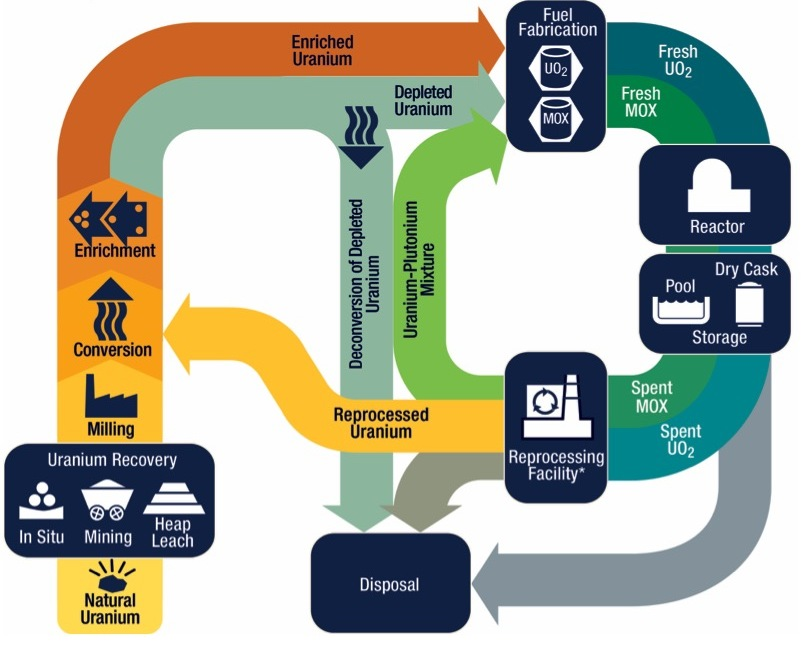
\includegraphics[width=0.8\textwidth]{images/The_Nuclear_Fuel_Cycle.jpg} 
        \caption[Nuclear Fuel Cycle]{Schematic representation of the nuclear fuel cycle from the 
mine to disposal.\cite{NuclearFuelCycle} }
        \label{FuelCycle}
\end{figure}

Nuclear fuel is mostly \ce{UO2(s)}. The useful fissile isotope 
is \ufis but it is only the 0.7\% of natural uranium being 99\% of it \unofis. For this 
reason, many reactors run 
uranium enriched in \ufis up to 1-3\%. Additionally, plutonium can also become fuel for several 
designs of reactors. This plutonium can be obtained from the dismantlement of thermonuclear 
bombs, also known as H-bombs, that use a 
plutonium fission explosion to initiate a fusion chain reaction of deuterium and tritium. 
Additionally,  during power generation in a nuclear power plant, the neutron 
capture of uranium generates plutonium. This plutonium can be recovered from 
spent uranium fuel, an extraction known as 
reprocessing. Plutonium and depleted uranium can be used in some nuclear reactors in the form 
of mixed oxides in a material known as \gls{mox}. Finally, there is a high interest in the 
substitution of uranium and plutonium fuels by thorium\cite{thorium} which would have 
significant advantages: it is more abundant and efficient than uranium, produces less harmful 
byproducts and cannot be used  to make weapons. But the most important feature of the thorium 
chain reaction is that there is no possibility of a meltdown like in Chernobyl making it much 
safer than the uranium alternative. Unfortunately thorium technology is still under development 
and while uranium remains cheap the incentives to fully develop thorium technologies are low. 
Figure \ref{FuelCycle} represents the cycle of uranium from the mine to its disposal.

High level radioactive waste is made by nuclear power plant residues
which are the result of the fission of the fuel. They contain unstable nuclei that  
emit alpha, beta or gamma radiation. Nuclear fuel is much more radioactive and dangerous when 
it has already been spent. For this reason 
reprocessing is a much more environmentally dangerous step than the actual power production. 
In spite of this, 
there has never been any accident in the handling and permanent storage of high level 
radioactive waste.

\begin{table}[h!]
\caption[Composition of spent nuclear fuel]{Typical composition of spent nuclear fuel from a 
uranium nuclear 
power plant.\cite{NuclearesLozano}}\label{comp}
\centering
{\small
\begin{tabular}{ll}
\toprule
95.6\% &$^{232}$U: 0.1-0.3\%; $^{234}$U: 0.1-0.3\%; $^{235}$U: 0.5-1.0\%; $^{236}$U: 
0.4-0.7\%; \unofis : rest \\
2.9\% &Stable elements.\\
0.9\% &Pu.\\
0.3\% &Cs and Sr (fission fragments).\\
0.1\% &I and Tc (fission fragments).\\
0.1\% &Long-lived fission fragments.\\
0.1\% &Np, Am and Cm (long-lived transuranium elements).\\
\bottomrule
\end{tabular}}
\end{table}


Reprocessing extracts uranium and plutonium from the waste to feed the reactor and separate 
radiotoxic elements for its permanent disposal. Spent nuclear fuel composition is summarized 
in Table \ref{comp}. The main problem of reprocessing is the complexity of the mixture 
including a wide variety of elements and isotopes some of them chemically very similar like the 
actinoids. 
If reprocessing is done, which is not always the case for economical reasons, it is done 
normally using the \gls{purex} method (Plutonium Uranium Redox 
EXtraction).\cite{NuclearesLozano,HERBST2011141,Katz2007-ch24} 

The PUREX method was developed as a part of the Manhattan project at the Oak Ridge National 
Laboratories and its initial goal was to purify plutonium for its use as a nuclear weapon 
detonant. The first step of PUREX is to dissolve the solid nuclear fuel pellets in 
concentrated nitric acid. Then Pu and U are extracted using liquid/liquid extraction. The 
original aqueous phase is exposed to a hydrocarbon phase in the presence of a complexating 
agent, mainly, tri n-butyl phosphine (\gls{tbp}):
\begin{align*}
&\ce{[UO_2*(H2O)5]^{2+}(aq) + 2NO3^-(aq) + 2TBP(org) <=> [UO_2(NO3)2*(TBP)2](org) }\\
&\ce{[Pu*(H2O)_n]^{4+}(aq) + 4NO3^-(aq) + 2TBP(org) <=> [Pu(NO3)4*(TBP)2](org) }
\end{align*}
TBP is highly selective for oxidation states VI and IV and virtually has no affinity for 
states III and V (Np(V), Am(III), Cm(III), etc.). The extraction is nearly 
quantitative and highly selective. The organic phase is then treated with reducing agents to 
reduce Pu(IV) to Pu(III) which is extracted with another aqueous phase with a very high yield. 
The resulting Pu and U solutions are then purified, evaporated and the actinoids are converted 
into oxides to be reused as nuclear fuel. The key chemical point in the 
process is the stability of \ce{[UO_2]^{2+}} and the chemical and electrochemical flexibility 
of the Pu ions. The original aqueous phase contains all the highly radioactive elements, most 
importantly highly radiotoxic actinoids like Cm, Am and Np.  Although the basic chemical ideas 
behind PUREX are simple, in practice it is a very complex chemical engineering process.

The final waste generated from PUREX contains the very radioactive but non-fissile 
nuclei including several transuranium actinoids (Np, Am and Cm mostly). This radioactive waste is 
the smallest by far in volume of all radioactive waste of industry but concentrates most of 
the sample radioactivity: 99.9\%. For this reason they are known as High Level Radioactive 
Waste 
(\gls{hlrw}).\cite{OECD-NEA-HLRW}

\section{High Level Radioactive Waste Permanent Storage}

HLRW is kept in waste pools close to the reprocessing or nuclear power plants allowing them to 
cool off with water acting as a radiation barrier. These materials 
can be then vitrified or solidified and introduced in stainless steel containers and allowed 
cooling for up to 50 years before their permanent disposal. The radioactive activity of the 
containers will remain terribly harmful for hundreds of thousands of years. 

Several solutions have been proposed to conceal for the centuries to come the HLRW: underground 
geological permanent storage, deep sea ground storage, glacier storage in Antartida, sending it 
to 
outer space or transmutation into harmless nuclei. Even though transmutation would be the ideal 
solution, unless major breakthroughs occur, Science is decades away from that kind of 
technology. 
The best agreed solution is storage in geological underground permanent 
disposal sites. Geological permanent storage sites are chambers dug deep underground in the rock 
where the containers will be stored safely for the centuries to come. The construction would 
be done in geologically stable locations and the rock would conceal the radioactive matter 
and its radiation. The rock acts as a passive barrier and also prevents any water from
leaking in or out of the repository. 

Most countries do have nuclear permanent disposal sites to keep mid and low level radioactive waste 
generated by the non-nuclear industry, research, radiomedicine etc. Nevertheless, even though the 
amount of HLRW has been growing since the beginnings of nuclear power production  a fully functional 
HLRW permanent geological disposal site is still missing. Many countries have 
plans to build it. Finland will be the first country to have a geological HLRW disposal 
site, Onkalo, 
in Posiva which is expected to become operative in 2023.\cite{OECD-NEA-HLRW}

The security of the facilities must be extreme. Specially because the nuclear containers remain hot 
for hundreds of years and are exposed to severe radiation damage. The sites should be air-tight 
particularly to prevent the entrance of water that could disperse the radioelements into the 
underground streams. 

\begin{figure}
     \centering
     \subfloat[a)]{{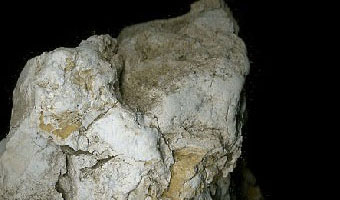
\includegraphics[width=7.5cm]{images/MMT_rock.jpg} }}%
     \\
     \subfloat[b)]{{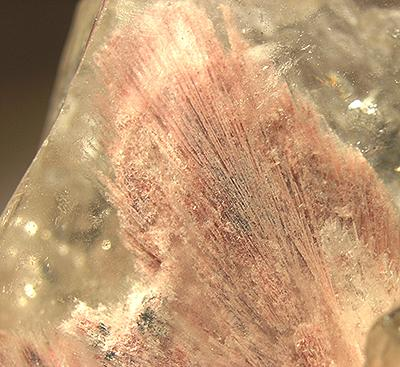
\includegraphics[width=7.5cm]{images/MMT_cris.jpg} }}%
     \caption[Montmorillonite clay minerals]{a) Montmorillonite clay rock. b) Montmorillonite 
clay crystals embedded in quartz.\cite{MMT_mac1,MMT_mac2}}
     \label{clay}
\end{figure}


\begin{figure}
     \centering
         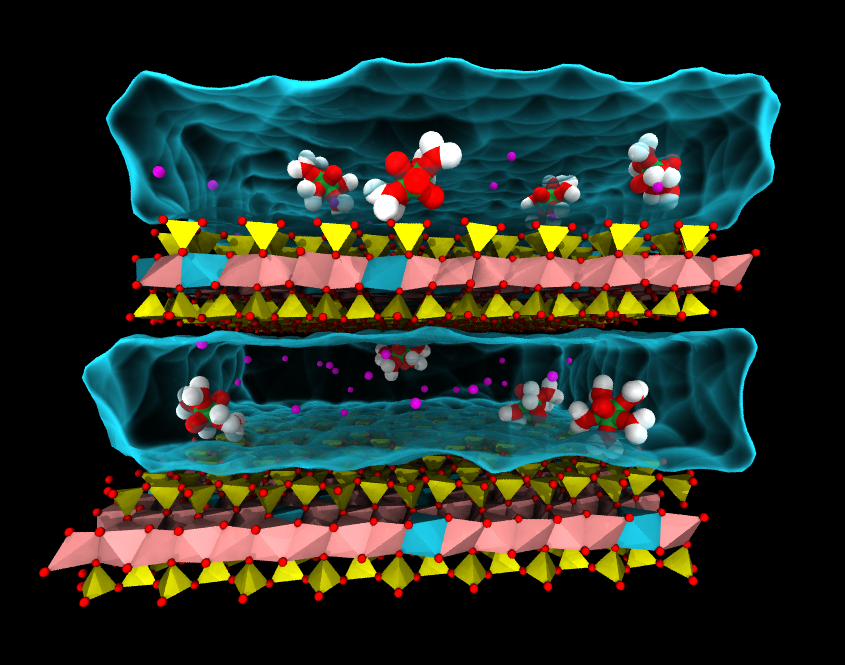
\includegraphics[width=0.8\textwidth]{images/clay} 
        \caption[Hydrated montmorillonite clay containing uranyl cations]{Unit cell of hydrated 
sodium montmorillonite clay containing uranyl hydrated ions, \ce{[UO2*(H2O)5]^{2+}}, in the 
interlayer. The water bulk water molecules are omitted and represented as a blue transparent 
surface. The uranyl cations are drawn with the ``licorice'' representation. \ce{SiO4} tetrahedra 
(yellow), \ce{AlO6} octahedra (pink) and \ce{MgO6} (blue) are represented as polyhedra. The atoms 
are colored as follow: O (red), H (white), \ce{Na^+} (purple) and U (green). }
        \label{clay2}
\end{figure}

Clays are particularly suited both as natural host rock or natural barrier for the permanent 
geological HLRW site and as liner material or artificial barrier to conceal the 
repository.\cite{Delage2010} The most used clay rock is bentonite which is primarily 
composed of montmorillonite clay (Figures \ref{clay} and \ref{clay2}). Bentonite is compacted 
and mixed with sand 
and serves as an 
artificial barrier surrounding the horizontal galleries which hold the HLRW. Clays are selected 
for three reasons: their high thermal conductance to dissipate the heat generated by the 
waste radioactivity, its low permeability to water and its high retention of radionucleides. 
This high retention of radioelements is due to their ionic exchange capability. If the
clay is exposed to a cation containing solution it would release its harmless \ce{Na+} cations and 
absorb radioactive cations such as actinyls.

\section{Hydrophobic Solvation}\label{sec:hydrophobicity}
In this section, we will make a small detour from the actinoids to talk about hydrophobic solvation 
which shall be relevant in the study of actinyl solvation and the development of the hydrophobicity 
and hydrophilicity fingerprint.

``Like dissolves like'' is one of the first concepts a chemist learns in relation to the 
solvation 
of compounds.\cite{reichardt2011solvents-ch1} It implies that solutes that are chemically like 
water 
will mimic water and be 
hydrophilic. Solutes that are not like water will ``dislike'' water and be 
hydrophobic. The classification of atoms and by extension molecules as hydrophilic and hydrophobic 
has traditionally been done based on chemical experience and heuristics which assign the character 
based on the chemical identity of the atoms. Hydrophobicity and hydrophilicity plays an important 
role in 
processes such as solvation, protein folding, micelle or membrane formation, phase transfer or 
crystallization.  

Hydrophobic solvation has several peculiarities. Hydrophobic compounds have a positive free energy 
of hydration, a negative entropy of hydration, a negative enthalpy of hydration and a large 
positive specific heat of hydration\cite{Harris2016,Ben-Amotz2016}. The word ``hydrophobic'' can 
generate the impression that the interaction of a hydrophobe with water should be repulsive and 
therefore its solvation enthalpy positive. Nevertheless, hydrophobic solutes interact through van 
der Waals interactions with water which are weak compared to water-water interactions but 
attractive. van der 
Waals interactions are non-di\-rec\-tio\-nal so water molecules are free to form a hydrogen 
bond 
network around the solute. Figure \ref{CH4} shows methane in liquid water and how the water 
molecules form their hydrogen bond network around the solute.

Hydrophobic solutes have the tendency to self-aggregate reducing their surface exposed to  
water. This self-assembly is known as the hydrophobic effect. Within chemistry and biochemistry it 
is common to talk about hydrophobic interactions or forces to describe the 
hydrophobic effect but this is misleading and should be avoided\cite{Cremer2017}. It seems to 
suggest 
that there is an intermolecular interaction ``special'' to these systems which have only regular 
van der Waals or hydrogen bond interactions. The hydrophobic effect is a water-mediated 
``self-sorting'' phenomenon. The free energy of water molecules is lower at bulk solution than on a 
hydrophobic molecule surface. The segregation of hydrophobic solutes reduces the amount of water at 
their surfaces producing an overall decrease of free energy of the system. 

The self-assembly \textit{is}
driven by a force, but it must be considered a force only in the ``potential of the 
mean force'' sense. In order words, if there 
is a free energy surface which is a function of a self-assembly collective variable its derivative 
can be 
considered the hydrophobic effect force.\cite{Ben-Amotz2016} Nevertheless, this terminology leads 
to misunderstandings and should ideally disappear. 

\begin{figure}
\centering 
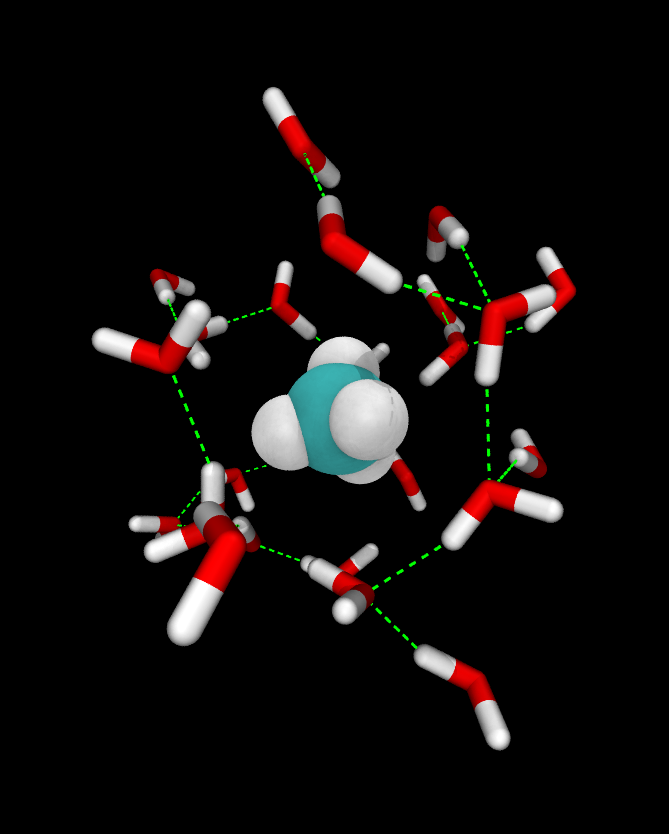
\includegraphics[width=7cm]{./images/CH4.png}
\caption[Hydration of \ce{CH4}]{Snapshot of a MD
simulation of methane in water. 
Only 
nearest water molecules are shown. The water molecule forms its hydrogen bond network around the 
cavity generated by methane in the solvent. }
\label{CH4}
\end{figure}

It has long been known that for small hydrophobic solutes at room temperature the entropic term 
dominates the free energy of 
solvation and is the reason for the low solubility of hydrophobic molecules in 
water.\cite{Chandler2005} This was explained theoretically in the works of Hummer et 
al\cite{garde1996origin,hummer1996information} on hydrophobic solvation. Their works started a body 
of theory known as ``Information Theory'' of hydrophobic solvation. Information Theory models the 
hydrophobic solute as a cavity in water. This cavity can be explicitly generated in solution by 
introducing a hard sphere particle or by the isomorphic problem of studying spontaneously generated 
cavities in water.

The cavity generated by hydrophobic solutes disrupts the hydrogen bond network of water decreasing 
the number of allowed microstates and thus the entropy of the solvent. Interestingly, this happens 
without affecting the average number of hydrogen bonds 
formed by the solvent around small 
solutes.\cite{Pratt1977,KaLum1999,Huang2001,Huang2002,Chandler2005} For this reason 
the hydration entropy of small hydrophobic \newline molecules correlates with molecular volume. 
This picture relates to the classical notion of hydrophobic solvation proposed by Frank and Evans 
in 
1945, the ``Iceberg'' model of hydrophobic solvation. In this model, the 
structure of water around a hydrophobic solute is reinforced and the dynamics slowed down by the 
formation of an ice-like cage of water molecules\cite{frank1945free}.

If the molecular size is high ($\sim$\SI{1}{\nano\meter}) a water/vapor-like interface is 
generated\cite{Willard2014} and the hydration entropy correlates with the 
molecular 
surface area instead of volume.\cite{Chandler2005} The reason is that water on the solute surface 
cannot form in this case the average number of hydrogen bonds it forms in solution.

Unlike hydrophobic solvation of small 
molecules at room temperature, the hydrophobic effect can be enthalpy driven, entropy driven or 
both\cite{Cremer2017,Chandler2005}. Quoting David Chandler: 

``The increase in molecular self-assembly of hydrophobic solutes with temperature is often cited as 
implying that hydrophobic interactions are entropic. Entropy does indeed contribute, but the
assembly process is driven by the difference between the entropically dominated solvation free 
energy of small molecules and the enthalpically dominated solvation free energy of large 
surfaces.'' \cite{Chandler2005}

\section{Systems Studied} 

The studies performed during this thesis are based on a simple scientific belief: 
fundamental understanding sheds light on applications. We study several systems important to 
the nuclear industry using fundamental science, for the sake of understanding, but bearing 
in mind the importance an applied scientist might give to our findings. For this reason we 
focus on systems that are interesting in themselves but also of potential relevance in waste 
reprocessing and storage or general actinoid chemistry. 

We studied four elements: uranium, neptunium, plutonium and americium. These four elements 
lie together in the actinoid or $5f$ row and are crucial in nuclear industry as fuels, 
dangerous waste or potential pollutants if accidents happened. We have studied their 
actinyl form, \ce{[AnO2]^{2+/+}} which correspond to oxidation states VI and V, and their main 
species in highly oxidizing and acidic aqueous media. Their study in solution is 
crucial because it is the form in which they are reprocessed and their dangerous mobile form 
if accidents were to occur. We also studied uranyl in clays to study its diffusion in 
the material and how the clay would slow down its diffusion compared to aqueous solution. 

A local example can be put forward with respect to accidents, not of the nuclear power
industry, but rather of the violent use of radioactivity. In 1966, two American military 
aircrafts crashed and 4 termonuclear plutonium bombs were dropped in Palomares (Almer\'ia) 
which is a 4 hour drive away from where I am writing this Thesis.\cite{palomares} Fortunately, only 
the conventional explosive of two of the bombs exploded and no nuclear explosion happened. 
Nevertheless, the explosion dispersed an aerosol of Pu in the nearby area. Although the bombs 
were recovered and part of the contamination cleaned, to this day regions around where the 
bombs landed are under strict nuclear control. One of the problems of Pu is its decay over time 
into Am which is much more volatile and radiotoxic than the rest of actinoids. For this kind of 
reasons, it is very important to understand the apparently obscure chemistry of americium in 
natural media such as clays or water.\cite{Katz2007-ch8}

Besides the nuclear industry, actinoids have a very interesting fundamental 
chemistry\cite{Pichon2017} in terms of bonding, electronic structure and reactivity. 
Understanding the chemistry of 
the compounds can help technological development. Neptunium as of today lacks any practical 
use, but who would have thought that \ce{^{241}Am} would be present in every household smoke 
detector due to its $\alpha$-emition (although they were banned in Spain in 2005). Also, 
though it might sound shocking, uranium is 
a 
naturally occurring element which is 40 times more abundant than silver. Therefore, knowledge 
of its speciation and chemistry in natural waters or clays is important even when its source 
is geological.

Experimental information on actinoids in solution is scarce and hard to 
obtain.\cite{Ions_in_sol_and_Marcus_2016,actinides_solution_v2,chemrev_Altmaier_2013} The 
reason for 
this is their radioactivity which requires 
the use of specialized techniques and specialized facilities.\cite{Pichon2017} 
Theoretical chemistry of actinoids gives many opportunities to study them in an 
inexpensive and safe way. This is the point of view adopted in this thesis: the studies here 
reported have been devoted to the 
computational chemistry of several actinoid cations and their actinyl forms but also in close 
relation to experiment, for example, in the simulation of EXAFS spectra. 

The first article of the compilation deals with the development of an \textit{ab initio} force 
field based on the hydrated ion model\cite{JPhysChem_ESM_1993,JChemPhys_ESM_1998} (\gls{him}) for the 
uranyl pentahydrate, \ce{[UO2*(H2O)5]^{2+}}, in 
solution. The force field allowed us to run classical molecular dynamics (\gls{md}) simulations 
and 
obtain 
interesting \newline in-solution properties of the complex. In particular: to describe the two 
solvation 
behaviors it 
exhibits as well as many spectroscopic, dynamic and thermodynamic properties. The second article 
extends the uranyl force field to the rest of studied actinyls: Np(V,VI), Pu(VI) and Am(VI). The 
simulations of cations reveal a great chemical analogy between them with some differences 
between the two oxidation states of neptunyl. The third article deals with the theoretical 
EXAFS 
 spectroscopy of aqueous actinyls. In particular, we compare theoretical EXAFS spectra to 
experiment and how increasing the level of theory of the reference quantum mechanical 
calculations has small 
structural effects with high spectroscopical impact. On the fourth article we used aqueous americium
MD simulations to interpret the experimental EXAFS spectrum of a Am(III)/Am(VI) 
mixture\cite{JRadioanNucChem_Riddle_2016} and to predict the EXAFS spectrum of a pure sample 
of Am(VI) in 
solution proposing the structural 
parameters of this hydrate. In the fifth article a hydrated ion-clay interaction potential is 
developed in 
order to run MD simulations of uranyl hydrated ions in a montmorillonite clay. We 
studied the diffusion of the uranyl cations within the clay and the effect of increasing the 
actinoid concentration in the interlayer. Metadynamics simulations were also run revealing the free 
energy surface of the uranyl cations as they diffuse in the aqueous interlayer. 

In a small detour from the actinoid project, we present as the final article the work done at the 
group of Prof. Michele Parrinello in Universitt\`a della Svizzera Italiana (Switzerland). 
During this 
six-month stay we developed a simple local fingerprint for hydrophobicity and hydrophilicity 
of 
atoms in complex solutes: from methane to amino acids. The fingerprint is inspired by the 
expansion of the entropy of a simple liquid in increasing terms of correlation order. 
We then 
used the fingerprint as a desolvation collective variable in a well-tempered metadynamics 
simulation of a host-guest system. In addition, the ability of the fingerprint to identify the 
hydrophobicity or hydrophilicity of the hydrated actinyl atoms was explored. 

\section{Literature Review}

I will now  review the literature of the field. For the sake 
of succinctness, the scope will be exclusively actinyl aqua-ions in solution or in montmorillonite 
clay in the context of statistical mechanics simulation. Many of the information left out has been 
reviewed elsewhere\cite{ChemSocRev_Wang_2012,dolg2015computational}.

For obvious reasons, the most studied of actinyl in the literature is uranyl, 
\ce{[UO2*(H2O)5]^{2+}}. It 
has been studied with all kinds of model hamiltonians from empirical force fields to 
Carr-Parrinello Molecular Dynamics (\gls{cpmd}) and even QM/MM.

The pioneers in its study in solution were  
Guilbaud and Wipff\cite{JMolStr_Wipff_1996,JPhysChem_Wipff_1993}. They developed an empirical 
interaction 
potential for uranyl with water using its free energy of hydration to validate the force 
field. In their MD simulations they were able to obtain coordination numbers, 
first shell distances as well as relative free energies of complexation to calixarene, a 
complexating macrocycle. The 
Guilbaud and Wipff non-polarizable model is still the most used in uranyl studies. 
Particularly, 
before this thesis it was the only model used in clay-uranyl simulations. In light of new free 
energy data Kerisit and Liu updated the model in 2013\cite{JPhysChemA_Kerisit_2013}. Empirical 
polarizable force fields have also been developed by Guilbaud et 
col.\cite{Nguyen2015,Duvail2019}. 

Two uranyl-water force fields based on QM calculations precede the one developed in this work. The 
first one was developed by the Gagliardi and Roos group\cite{JACS_Roos_2005} using the polarizable 
NEMO approach\cite{NEMOJPC90}. The force field was parametrized with CASPT2 calculations of the 
uranyl monohydrate, 
\newline\ce{[UO2*(H2O)]^{2+}}. This model underlines the importance of charge transfer to the 
first 
solvation shell. The second and more 
recently developed force field was published by Maginn et 
al.\cite{JPhysChemB_Tiwari_2012} 
Their reference potential energy surface was obtained including four water molecules in the uranyl 
first shell to capture many-body effects and polarization in a non-polarizable framework. With this 
effective two-body 
model they studied a variety of 
structural and dynamic properties of 
uranyl hydration.\cite{JPhysChemB_Tiwari_2012,PhysChemChemPhys_Tiwari_2014}

\textit{Ab initio} MD simulations have also been employed. Bühl et al. ran 
CPMD simulations on aqueous uranyl obtaining interesting results concerning the 
dissociation of a water molecule out of the uranyl aqua-ion.\cite{JACS_Buhl_2005} They 
found a clear dominance of the pentahydrate complex over the tetrahydrate. Nichols et al. 
ran similar simulations and were able to use ensemble configurations to generate an EXAFS 
spectrum that reproduced remarkably well the 
experiment.\cite{JChemPhys_Nichols_2008} The system has also 
been studied employing QM/MM simulations by Frick et al. who calculated
angularly resolved radial distribution functions (\gls{rdf}).\cite{JPhysChemA_Frick_2009} 

Although the literature regarding uranyl molecular dynamics is abundant, the rest of actinyls have 
not received as much attention. The reason for this is that the 
chemical analogy between uranyl and the rest is high except for spectroscopical and magnetic
properties. The only classical force 
field for actinyls different than uranyl was developed by Maginn's 
group\cite{PhysChemChemPhys_Pomogaev_2013,PhysChemChemPhys_Tiwari_2014}. They extended their 
methodology for uranyl adding the specificity of the particular actinoid by changing its 
partial charges, bond bending and bond stretching  parameters in accordance to quantum 
chemical 
calculations. They found all the actinyls remarkably similar in terms of hydration. The 
other study was carried out by Odoh et al.\cite{JPhysChemA_Odoh_2013} They did 
CPMD-metadynamics simulations on \ce{[PuO2]^{2+/+}} studying the relative stabilities of their 
coordination numbers.

Clay classical MD simulations have a long history. To the best of our knowledge, 
the first interaction potential for clays was developed by Skipper et al. in 
1989 using semiempirical partial charges.\cite{skipper1989computer} The potential was initially 
used to study water (MCY model\cite{MCY}) at a talc surface but later allowed the study of more 
complex 
problems\cite{JACS_Refson_2000,JChemPhys_Skipper_1991}. The state-of-the-art clay force field is 
the \textit{clayFF} force field which has been cited over a thousand 
times.\cite{clayFF_JPhysChemB_Cygan_2014} This intuitively named force field, describes the 
clay as a set of charged Lennard-Jones spheres which by means of non-bonded interactions conserve 
the clay structure reproducing several experimental properties. The \textit{clayFF} allows the 
study of many hydrated and dehydrated clays, hydroxides and oxyhydroxides including its internal 
dynamics since it allows the aluminosilicate to be flexible. This force field will be used in this 
work to model montmorillonite clay. More recently, a polarizable clay force field has been 
proposed\cite{tesson2016classical}. The literature of aluminosilicate MD
simulations is very 
rich and is summarized in the following 
reviews.\cite{JMatChem_Cygan_2009,MolSimClayMin_HandbookofClayScience_Cygan_2013_v2}

The theoretical study of uranyl cations in montmorillonite clay has a significant amount of 
literature. Most of it refers to the study of the cation adsorbed on the outer pores of the clay 
particles exposed to 
bulk solution\cite{PhysChemChemPhys_Greathouse_2005,EnviSciTech_Greathouse_2006,JHazMat_Yang_2013,
JHazMat_Liu_2013,MolSim_Cygan_2014,
InorChemFronteirs_Zhang_2015} and only two refer to uranyl inside the clay interlayers. 
\cite{ClayMinSoc_Zaidan_2003,ClayMinSoc_Greathouse_2005} 

The first study was done by Zaigan et al. who studied uranyl in montmorillonite interlayers by means 
of Monte Carlo simulations. They used the Wipff and Guilbaud model for 
uranyl\cite{JMolStr_Wipff_1996,JPhysChem_Wipff_1993} and clay interaction potential of Skipper 
et al\cite{JChemPhys_Skipper_1991}. They obtained the interlayer spacing of the uranyl 
containing clay as a function of interlayer hydration, the dynamics of the uranyl axis 
orientation, the z-density profiles and uranyl radial distribution functions. The second study 
was done in 2005 by the same authors updating the simulation to interpret XAS 
spectra.\cite{ClayMinSoc_Greathouse_2005} After these two initial works and until this 
thesis, the uranyl clay simulations dealt with the adsorption of the cation in bulk-solution 
exposed surfaces of the clay. The majority of pore-uranyl clay simulations used a combination 
of the \textit{clayFF} and the Guilbaud-Wipff
model for uranyl. In this set of articles a variety of effects have been studied 
in this system: the influence of 
electrolyte concentration in the 
pore\cite{PhysChemChemPhys_Greathouse_2005,EnviSciTech_Greathouse_2006, 
InorChemFronteirs_Zhang_2015,MolSim_Cygan_2014} including coordinating counter ions like 
carbonate\cite{PhysChemChemPhys_Greathouse_2005,EnviSciTech_Greathouse_2006}, adsorption constants 
to the surface\cite{EnviSciTech_Greathouse_2006,PhysChemChemPhys_Greathouse_2005}, the z-density 
distribution\cite{InorChemFronteirs_Zhang_2015,JHazMat_Liu_2013, 
JHazMat_Yang_2013,EnviSciTech_Greathouse_2006}, the average surface charge 
density\cite{InorChemFronteirs_Zhang_2015}, superficial uranyl and water
diffusion\cite{JHazMat_Liu_2013} and superficial uranyl orientation\cite{MolSim_Cygan_2014}.



\bibliographystyle{achemso}
\bibliography{./library,./extrabib}
